% ! TeX root = ../../main.tex
\chapter{Background e contesto}
Nel settembre degli anni 2000 venne adottata la Dichiarazione del Millennio delle Nazioni Unite (United Nations Millennium Declaration) \cite{millennium_declaration} da parte degli stati membri che, considerando alcuni principi considerati fondamentali per le relazioni internazionali nel ventunesimo secolo (libertà, uguaglianza, solidarietà, tolleranza, rispetto per la natura, responsabilità condivisa), identificarono otto obiettivi principali da raggiungere entro il 2015 chiamandoli Millenium Development Goals (MDGs); questi comprendevano:
\begin{description}
    \item[Goal 1] Sradicare l'estrema povertà e la fame
    \item[Goal 2] Raggiungere una educazione primaria universale
    \item[Goal 3] Promuovere l'uguaglianza di genere e potenziare le donne
    \item[Goal 4] Ridurre la mortalità infantile
    \item[Goal 5] Migliorare la salute materna
    \item[Goal 6] Combattere HIV/AIDS, Malaria e altre malattie
    \item[Goal 7] Garantire la sostenibilità ambientale
    \item[Goal 8] Instaurare una partnership globale per lo sviluppo
\end{description}

Come proseguimento del Millenium Declaration nel 2015 le Nazioni Unite hanno elaborato e sottoscritto un nuovo programma denominato Agenda 2030 \cite{agenda2030}, contenente 169 traguardi raggruppati in 17 Obbiettivi per lo sviluppo Sostenibile (Sdgs, \ref{sec:sdgs}) con il fine di porre una buona base, condivisa da tutti i paesi membri, da cui partire per costruire un mondo sostenibile dal punto di vista ambientale, economico e sociale.
%
Ciascun stato membro è tenuto a sviluppare un strategia Nazionale e a questo proposito l'Italia ha istituito la Cabina di regia "Benessere Italia", un organo della Presidenza del Consiglio, che si occupa di coordinare, monitorare, misurare e opportunamente migliorare le politiche applicate dai Ministeri per l'attuazione della Strategia Nazionale di Sviluppo Sostenibile (SNSvS) \cite{SNSvS}.

Si tratta di una sfida globale che richiede il coinvolgimento non solo dei governi degli stati membri ma anche delle componenti della società come imprese private e pubbliche, società civili e operatori della informazione e cultura.

In questa ottica nel 2016 si è formata l'Alleanza Italiana per lo sviluppo Sostenibile (ASviS) \cite{asvis} su iniziativa della fondazione UniPolis e dell'Università di Roma \enquote*{Tor vergata}, con l'obiettivo di diffondere la cultura dello sviluppo sostenibile, facendo accrescere la consapevolezza dell'importanza dell'Agenda 2030.
Questa associazione vede a oggi una partecipazione di oltre 300 soggetti che si occupano di tematiche riconducibili agli Obiettivi di Sviluppo Sostenibile; fra gli aderenti alla alleanza vi sono associazioni, enti di diritto pubblico, università (fra queste anche l'Università di Bologna), enti e centri di ricerca pubblici e privati e tante altre organizzazioni della società civile italiana senza scopo di lucro \cite[Aderenti alla ASviS]{aderenti_asvis}. 
%
%
\section{Sostenibilità ed Ecosostenibilità}
\section{Definizione}
%
%
\section{Sdgs}
\label{sec:sdgs}
Gli Sdgs (Sustainable Development Goals)\cite{agenda2030}, in italiano Obiettivi per lo sviluppo sostenibile sono obiettivi principali da ambire e raggiungere da ogni stato membro e le sue componenti della società entro il 2030. Imprese private e pubbliche, operatori della informazione e società civili sono coinvolte in questo ambizioso progetto andando ad agire concretamente ad esempio per ridurre le disuguaglianze, sconfiggere la fame, lottare contro il cambiamento climatico e raggiungere una parità di genere.
Di seguito i 17 Obiettivi per lo sviluppo sostenibile e le loro grafiche (Figura \ref{fig:sdgs}):
\begin{description}
    \item[Goal 1] Sconfiggere la povertà
    \item[Goal 2] Sconfiggere la fame
    \item[Goal 3] Salute e benessere
    \item[Goal 4] Istruzione di qualità
    \item[Goal 5] Parità di genere
    \item[Goal 6] Acqua pulita e servizi igienico-sanitari
    \item[Goal 7]  Energia pulita e accessibile
    \item[Goal 8] Lavoro dignitoso e crescita economica
    \item[Goal 9]  Imprese, innovazione e infrastrutture
    \item[Goal 10] Ridurre le disuguaglianze
    \item[Goal 11] Città e comunità sostenibili
    \item[Goal 12] Consumo e produzione responsabili
    \item[Goal 13] Lotta contro il cambiamento climatico
    \item[Goal 14] Vita sott’acqua
    \item[Goal 15] Vita sulla Terra
    \item[Goal 16] Pace, giustizia e istituzioni solide
    \item[Goal 17] Partnership per gli obiettivi
\end{description}
%
\begin{figure}[h]
    \centering
    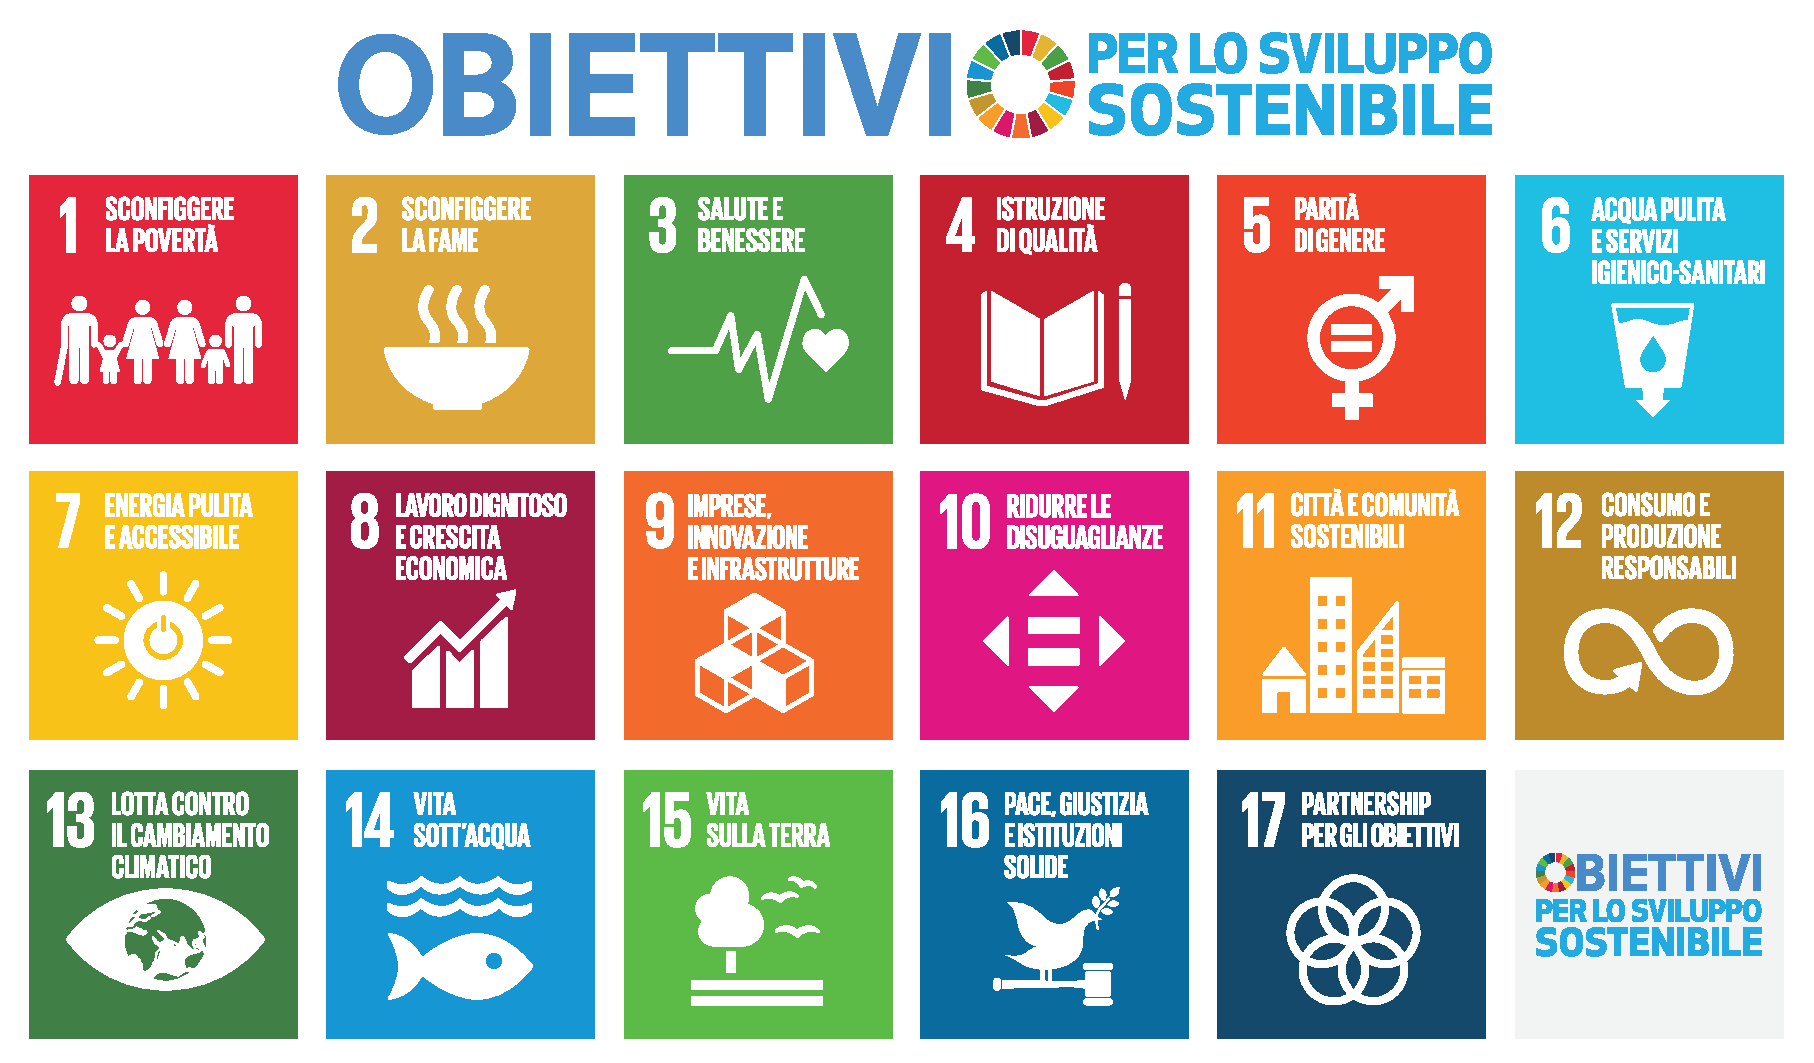
\includegraphics[width=\textwidth]{img/SDG_Poster.png}
    \caption{Grafiche dei 17 Obiettivi per lo sviluppo Sostenibile}
    \label{fig:sdgs}
\end{figure}
%
%
\section{Progetto Remade}
L'Università di Bologna da diversi anni ha intrapreso un percorso di dematerializzazione dei processi amministrativi e didattici con l'obbiettivo di ridurre l'utilizzo di carta favorendo mezzi e strumenti digitali.
%
Questo ambizioso percorso si intreccia fortemente con il progetto ReMade (REplanting for Monitoring Accomplishment of DEmaterialization, \cite{remade_project}) che nasce dall'obiettivo dell'Ateneo, con la collaborazione del CESIA, DICAM e DISI Sustainable ICT LAb, di potenziare l'effetto della riduzione di uso di carta nei processi amministrativi e di comunicazione (processo di dematerializzazione) convertendo questo risparmio nella piantumazione proporzionale di alberi negli spazi verdi.

\textcolor{red}{TODO: 
ATTIVITÀ
Oltre alla piantumazione di nuove alberature, i risultati virtuali (meno carta) e reali (più alberi) saranno diffusi attraverso una web app per affiancare, all'effetto sull'ambiente, un aumento di consapevolezza e competenza da parte della comunità Unibo.}

Con questo progetto l'Ateneo contribuisce a tre degli obiettivi per lo sviluppo sostenibile (Figura \ref{fig:remade_dgs}) che riguardano le città e comunità sostenibili (Goal 11), la lotta contro il cambiamento climatico (Goal 13) e la vita sulla terra (Goal 15); infatti la piantumazione di nuovi alberi porta inevitabilmente a diversi benefici come la riduzione della temperatura, rimozione d'inquinanti atmosferici e miglioramento dello stile di vita e vivibilità delle città.
%
\begin{figure}
    \centering
    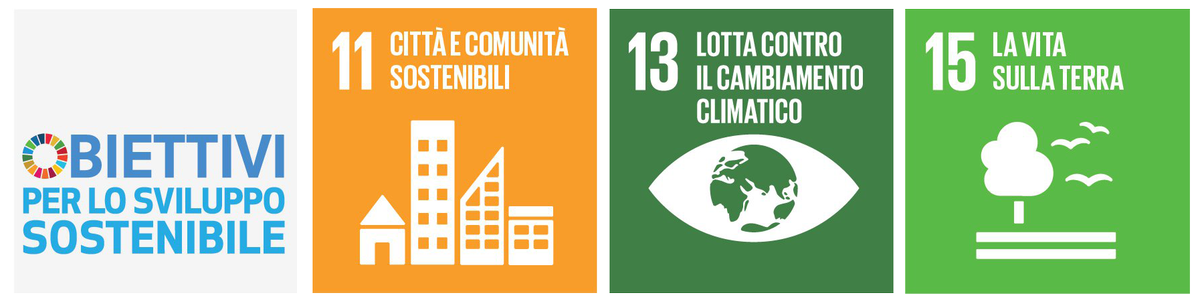
\includegraphics[width=\textwidth]{img/sdg_remade.png}
    \caption{Obiettivi Agenda 2030 sostenuti dal progetto ReMade}
    \label{fig:remade_dgs}
\end{figure}
%
\section{Motivare gli utenti}
Considerando la diffusione dei risultati ottenuti (meno carta e più alberi)del progetto ReMade e il desiderio di aumentare la consapevolezza e competenza sul tema da parte della comunità Unibo si ritiene necessario creare interesse e stimolare gli utenti attraverso meccanismi come la \enquote{Gamification} e i \enquote{Serious Game}.
%
\subsection{Gamification}

% Sono stati svolti diversi studi e ricerche che si intrecciato con la disciplina delle Human Computer Interaction che tendono appunto a scoprire e definire linee guida da utilizzare per sfruttare gli aspetti principali dell'intrattenimento e ricreativi dei videogiochi in contesti e applicazioni che non sono videogiochi.
% Per motivare gli utenti quindi si possono mettere in atto diverse strategie come la gamification che portano l'utente a una continua sfida personale e comunitaria con la possibilità di ottenere premi e o riconoscimenti.

Il fenomeno della gamification consiste nel portare aspetti principali dei videogiochi, come il concetto di punteggio e di livello, in contesti non prettamente di gioco in modo da migliorare l'esperienza e il coinvolgimento dell'utente.

% da collerare i due discorsi
Nella vita di tutti i giorni senza accorgercene siamo stimolati e invogliati ad andare in un determinato negozio o utilizzare un determinato mezzo di trasporto per accumulare punti convertibili in uno sconto, un omaggio o un viaggio gratuito.
%
\subsection{Serious game}

%
\section{Extended Reality}

\subsection{Realtà aumentata}

\subsection{Realtà virtuale}
\subsection{Mixed reality}
%
\section{Integrazione tra diversi tipi di device}
\section{Integrazione tra totem e smartphone}